


\tikzset{every picture/.style={line width=0.75pt}} %set default line width to 0.75pt        

\begin{tikzpicture}[x=0.75pt,y=0.75pt,yscale=-1,xscale=1]
%uncomment if require: \path (0,300); %set diagram left start at 0, and has height of 300

%Rounded Rect [id:dp3454362135099034] 
\draw   (203,113.4) .. controls (203,105.45) and (209.45,99) .. (217.4,99) -- (282.1,99) .. controls (290.05,99) and (296.5,105.45) .. (296.5,113.4) -- (296.5,156.6) .. controls (296.5,164.55) and (290.05,171) .. (282.1,171) -- (217.4,171) .. controls (209.45,171) and (203,164.55) .. (203,156.6) -- cycle ;
%Straight Lines [id:da8670184653139519] 
\draw    (232.5,128) -- (175.5,128.97) ;
\draw [shift={(173.5,129)}, rotate = 359.03] [color={rgb, 255:red, 0; green, 0; blue, 0 }  ][line width=0.75]    (10.93,-3.29) .. controls (6.95,-1.4) and (3.31,-0.3) .. (0,0) .. controls (3.31,0.3) and (6.95,1.4) .. (10.93,3.29)   ;

%Image [id:dp1573774251550818] 
\draw (329.75,151.22) node  {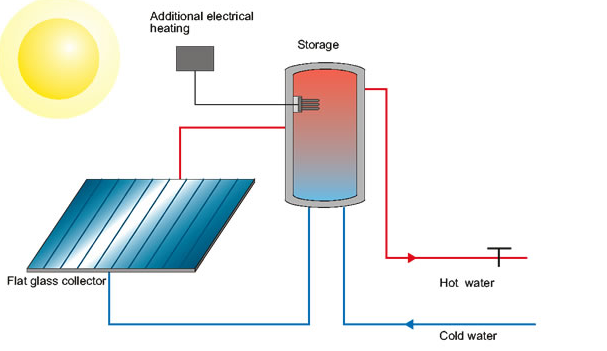
\includegraphics[width=391.13pt,height=232.5pt]{5.png}};
%Straight Lines [id:da756821456781489] 
\draw    (360.5,151.22) -- (442.5,150.24) ;
\draw [shift={(444.5,150.22)}, rotate = 539.3199999999999] [color={rgb, 255:red, 0; green, 0; blue, 0 }  ][line width=0.75]    (10.93,-3.29) .. controls (6.95,-1.4) and (3.31,-0.3) .. (0,0) .. controls (3.31,0.3) and (6.95,1.4) .. (10.93,3.29)   ;


%Straight Lines [id:da9580285561891552] 
\draw    (228.5,102.22) -- (302.5,101.24) ;
\draw [shift={(304.5,101.22)}, rotate = 539.25] [color={rgb, 255:red, 0; green, 0; blue, 0 }  ][line width=0.75]    (10.93,-3.29) .. controls (6.95,-1.4) and (3.31,-0.3) .. (0,0) .. controls (3.31,0.3) and (6.95,1.4) .. (10.93,3.29)   ;

%Straight Lines [id:da9281060785864365] 
\draw    (389.5,67.22) -- (430.5,67.22) ;
\draw [shift={(432.5,67.22)}, rotate = 180] [color={rgb, 255:red, 0; green, 0; blue, 0 }  ][line width=0.75]    (10.93,-3.29) .. controls (6.95,-1.4) and (3.31,-0.3) .. (0,0) .. controls (3.31,0.3) and (6.95,1.4) .. (10.93,3.29)   ;

%Straight Lines [id:da47053369422446445] 
\draw    (261.5,79.22) -- (294.5,79.22) ;
\draw [shift={(296.5,79.22)}, rotate = 180] [color={rgb, 255:red, 0; green, 0; blue, 0 }  ][line width=0.75]    (10.93,-3.29) .. controls (6.95,-1.4) and (3.31,-0.3) .. (0,0) .. controls (3.31,0.3) and (6.95,1.4) .. (10.93,3.29)   ;

%Shape: Circle [id:dp11314595015500317] 
\draw  [color={rgb, 255:red, 0; green, 0; blue, 0 }  ,draw opacity=1 ][fill={rgb, 255:red, 155; green, 155; blue, 155 }  ,fill opacity=1 ] (532.5,92.75) .. controls (532.5,88.19) and (536.19,84.5) .. (540.75,84.5) .. controls (545.31,84.5) and (549,88.19) .. (549,92.75) .. controls (549,97.31) and (545.31,101) .. (540.75,101) .. controls (536.19,101) and (532.5,97.31) .. (532.5,92.75) -- cycle ;

% Text Node
\draw (463,133) node   {$kA_{t}( T_{cont} -T_{env})$};
% Text Node
\draw (193,97) node   {$A_{c}( I_{env})$};
% Text Node
\draw (474,48) node   {$m( T_{cont} -T_{in})$};
% Text Node
\draw (339,116) node   {$T_{cont}$};
% Text Node
\draw (568,89) node   {$T_{env}$};
% Text Node
\draw (539,278) node   {$T_{in}$};
% Text Node
\draw (276,60) node   {$P_{aux}$};
% Text Node
\draw (540,217) node   {$T_{cont}$};


\end{tikzpicture}
